\chapter{Introduzione}
\section{Premessa}
Oggigiorno, la maggior parte dei PC utilizza sistemi operativi senza patch e/o senza alcuna sicurezza dietro un \textit{firewall}, rendendoli facili prede per attacchi diretti, orchestrati da malintenzionati, e/o per attacchi di tipo indiretto, mascherati dietro programmi che l'utente usa costantemente (vedi reti \textit{P2P}).\\
Con l'incremento delle connessioni a banda larga si ha avuto anche un incremento del numero di potenziali vittime di attacchi, con cui i malintenzionati traggono beneficio dalla situazione, utilizzandola a loro vantaggio, sfruttando anche l'automatizzazione di tecniche per la scansione di porzioni della rete che semplifica la ricerca di sistemi vulnerabili. Una volta che un vasto numero di macchine sono state infettate, esse entrano a far parte di ``una rete di macchine compromesse che posso essere controllate da remoto\footnote{Provos Niels, Holz Thorsten (2007).}'', chiamata una \textbf{botnet}.\\
Una \textit{botnet} consiste di tre elementi principali che sono i bot (cio\`e le macchine infettate che ne fanno parte), il \textit{command and control server} (C\&C - da cui ogni bot riceve istruzioni e con cui il malintenzionato ha privilegi amministrativi remoti su tutte le macchine infette) e un \textit{botmaster}; si basa, inoltre, su quattro concetti chiave:
\begin{enumerate}
\item le \textit{botnet} sono reti, quindi sistemi in cui la comunicazione \`e importante;
\item le macchine che fanno parte di una \textit{botnet} sono, tipicamente, partecipanti ignari;
\item i \textit{bot} sono controllabili da remoto, permettendo di fare rapporto o ricevere ordini da una struttura C\&C (centralizzata o decentralizzata);
\item i \textit{bot} sono controllati da persone con intenti malevoli che fanno capo a qualche forma di attivit\'a illegale, come la diffusione di un virus, effettuare attacchi DDos, spam, \dots .
\end{enumerate}
Se il proprio computer diventa parte di una botnet, i criminali creando un scenario di vero e proprio pericolo per ogni infrastruttura IT, in quanto i bot verranno utilizzati con intenzioni malevole.

\vspace*{1cm}
\section{HTTP Botnet}
\begin{figure}[h]
        \centering
		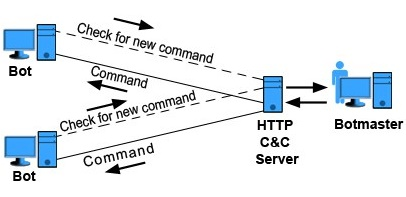
\includegraphics[width=0.5\linewidth]{./imgs/botnet1999}
        \caption{Struttura di una botnet}
        \label{strutturabotnet}
\end{figure}
Quando il protocollo HTTP nacque nel 1999, nessuno avrebbe mai pensato che sarebbe stato utilizzato per le botnet. 
La prima generazione di botnet usava l'\textit{Internet Relay Chat} (IRC\footnote{Protocollo di messaggistica istantanea su Internet, che consente sia la comunicazione diretta fra due utenti, che il dialogo contemporaneo di gruppi di persone raggruppati in stanze di discussione dette canali.}) e relativi canali per instaurare un meccanismo di ``controllo e comando''. I bot IRC seguono lo stesso approccio PUSH di quando ci si unisce ai canali, rimanendo connessi. Essi si connettono ai server IRC e ai canali che sono stati selezionati dal \textit{botmaster} e attendono comandi. 
Invece di rimanere connessi, i bot HTTP controllano periodicamente per aggiornamenti oppure nuovi comandi: questo modello \`e detto di PULL e continua ad intervalli regolari definiti dal botmaster, il quale, usa il protocollo HTTP per nascondere le proprie attivit\'a tra il normale flusso web, riuscendo ad evitare facilmente i metodi di rivelazione come i \textit{firewall}. 

\vspace*{1cm}
\section{Obiettivo}
L'obiettivo \`e quello di sviluppare un software per workstation che definisca bot in grado di contattare delle URL a cui sono associate una serie di variabili:
\begin{enumerate}
\item definizione della periodicit\'a del contatto fissa o variabile in un intervallo temporale;
\item definizione del numero massimo di contatti per ciascuna URL;
\item definizione di una modalit\'a di ``\textit{sleep}'', intesa come insieme di condizioni in cui non viene effettuata nessuna azione ;
\item definizione di uno user-agent ``\textit{custom}'';
\item definizione di un indirizzo e porta di ``\textit{proxy}'' pubblico.
\end{enumerate}
Tali definizioni saranno effettuate o tramite \textit{file .txt} oppure tramite \textit{Graphic User Interface} (GUI).\\
Inoltre, contatti alle URL con i loro dettagli, variabili di configurazione, \textit{timestamp} dei contatti, Sistema operativo utilizzato e \textit{browser} presenti sulla macchina
saranno opportunamente salvati in un \textit{file log}.

\vspace*{1cm}
\section{Struttura della relazione}
L'analisi, progettazione e sviluppo del progetto inizia con un'esposizione del programma implementato, spiegandone la logica, ed esponendo il tentativo di conferire una modalit\'a di utilizzo immediata, con poche piccole azioni. Nel capitolo successivo si parler\'a degli elementi principali del progetto e tutto ci\`o che li riguarda, evidenziandone il processo di analisi. A seguire, un capitolo dedicato alle metodologie utilizzate per la creazione dei bot facenti parti della rete. Infine, l'ultimo punto, \`e quello dell'analisi dei casi di test effettuati per un corretto funzionamento del programma.